%4. Problemraum (Prototyp, Testaufbauten, bestehende Software)
\chapter{Understanding the Problem Space}
\label{chap:understanding-the-problem-space}
In order to provide a satisfying solution to the problem at hand, the problem itself and the environment it occurs in must be researched. This chapter aims to explore and examine the problem space, resulting in a set of artifacts (namely a domain model and a set of requirements) that aid in understanding the context and designing an appropriate solution. First, a prototypical network proxy is designed and implemented in section \ref{sec:prototypical-implementation} to get an understanding of the problems and challenges involved in designing, implementing and using such software. Based on these experiences, interviews with experts in penetration testing are conducted and evaluated in section \ref{sec:interviews} to get a proper understanding of their everyday work and resulting problems. Lastly, existing software that aims to intercept communication for various scenarios and technologies is examined in section \ref{sec:analysis-existing-software}, compared to each other and their usefulness for the problem-specific scenarios is assessed.

\section{Prototypical Implementation}
\label{sec:prototypical-implementation}
The prototype was designed to be able to handle two scenarios; a simple and a complex one. Complexity was evaluated by the amount of communication protocols and steps involved. The goal of this section was to implement a prototype that could be used to intercept communication between an \ac{IoT} device and its cloud service as shown in figure \ref{fig:network-communication-diagrams}.   

\begin{figure}%
    \centering
    \subfloat[\centering Regular communication between an \ac{IoT} device and a cloud service.]{{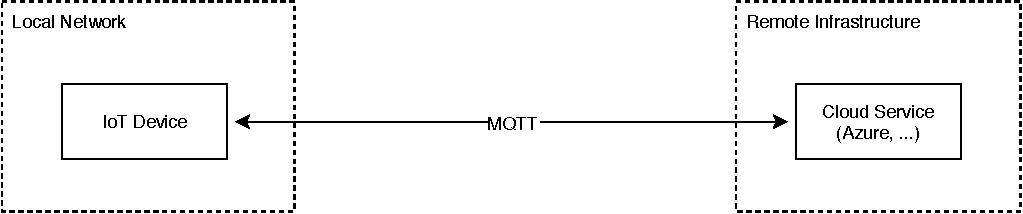
\includegraphics[width=10cm]{img/ch04/Setup - 1 Regular.pdf} }}%
    \qquad
    \subfloat[\centering Communication intercepted by a \ac{MITM} proxy.]{{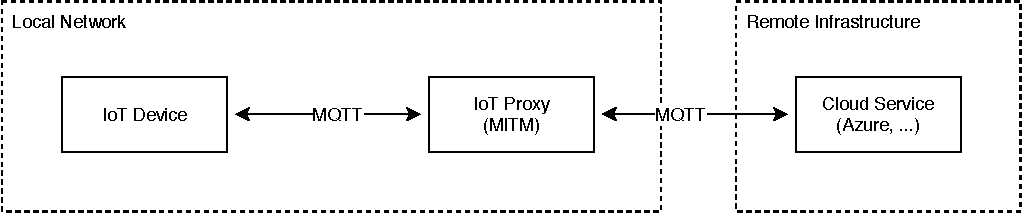
\includegraphics[width=10cm]{img/ch04/Setup - 2 Pentesting.pdf} }}%
    \caption{Installing a \ac{MITM} proxy to intercept network communication for penetration testing.}%
    \label{fig:network-communication-diagrams}%
\end{figure}

\subsection{Simple Scenario: ICS Modbus TCP}
% Hardware Setup
% Communication

\subsection{Complex Scenario: AWS IoT}
% Hardware Setup
% Communication



\subsection{Requirements}
%TODO: Move overscoped requirements to design of the second prototype?
To be able to operate in both of the aforementioned scenarios, the prototype had to implement a set of functional requirements:
\begin{itemize}
    \item [\textbf{F1}] \textbf{Protocols:} The software must implement parsing/crafting messages/packets of the following communication protocols: \ac{HTTP}, \ac{WS}, \ac{MQTT} and Modbus \ac{TCP}. \\
    \textit{Fit criterion: TBD} %TODO: Do lol 
    \item [\textbf{F2}] \textbf{Network Stacks:} The software must provide an interface to the user where they can specify which communication protocols are to be used and whether and how they are stacked (further referred to as \emph{network stack}).\\
    \textit{Fit criterion: The software processes a configuration file that lets users specify which protocols to be used and whether/how they are stacked.} 
    \item [\textbf{F3}] \textbf{State Machine:} The software must provide an interface for the user to specify when to switch to using another network stack, represented using state machines.\\
    \textit{Fit criterion: The software processes a configuration file that lets users specify when to switch between network stacks.}
    \item [\textbf{F4}] \textbf{Integration:} The software shall provide interfaces for integration of third-party software.\\
    \textit{Fit criterion: The software allows sending requests/responses to \enquote{Burp Suite} for manipulation.} %TODO: Do lol
    \item [\textbf{F5}] \textbf{Scripting:} The software shall provide scripting capabilities for automated manipulation of messages/packets.\\
    \textit{Fit criterion: Users can define script-snippets to be executed on messages/packets.} %TODO: Do lol
\end{itemize}

The following non-functional requirements were defined:

\begin{itemize}
    \item [\textbf{N1}] \textbf{Extensibility:} To allow for future implementation of further communication protocols the software shall be implemented in a modular fashion.
    \item [\textbf{N2}] \textbf{Platform Compatibility:} In order to support a broad spectrum of target platforms, the software shall be implement plattform-independently.
\end{itemize}

Due to this implementation serving as a prototype and being of an academic nature, no specific constraints were defined. It was developed strictly ignoring aspects of usability and stability as it should not be used in production environments but in laboratories exclusively.

\subsection{Design}
% Overall
% Network Stack
\begin{figure}[t]
    \centering
    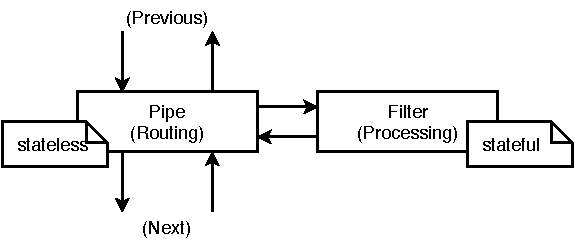
\includegraphics[width=6cm]{img/ch04/Architecture - Pipes and Filters.pdf}
    \captionof{figure}{Statemachine of \ac{AWS} \ac{IoT} communication}
    \label{fig:aws-statemachine}
\end{figure}

% TODO: References Pipes & Filters \ref{fig:app-diag-pipesfilters-1} \ref{fig:app-diag-pipesfilters-2}

% Statemachine
\begin{figure}[t]
    \centering
    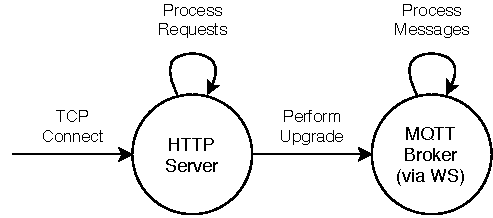
\includegraphics[width=6cm]{img/ch04/Statemachine 2.pdf}
    \captionof{figure}{Statemachine of \ac{AWS} \ac{IoT} communication}
    \label{fig:aws-statemachine}
\end{figure}
% Reference: https://aws.amazon.com/blogs/aws/aws-iot-cloud-services-for-connected-devices/


\subsection{Implementation}

\subsection{Insights Gained}


%\begin{figure}[t]
%    \centering
%    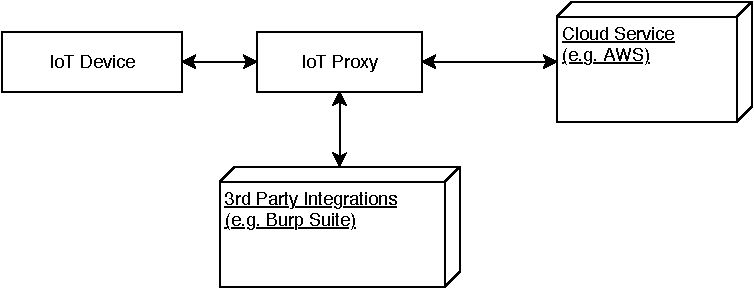
\includegraphics[width=6cm]{img/ch04/Architecture - Simple.pdf}
%    \captionof{figure}{High-level Software Architecture}
%    \label{fig:high-level-software-architecture}
%\end{figure}

%\begin{figure}[t]
%    \centering
%    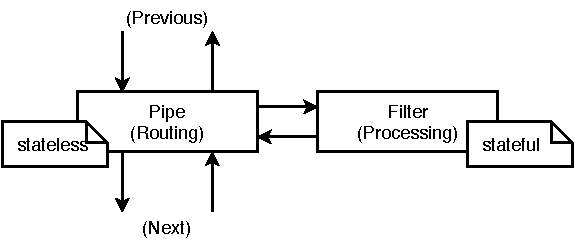
\includegraphics[width=6cm]{img/ch04/Architecture - Pipes and Filters.pdf}
%    \captionof{figure}{"Pipes and Filters" Design Pattern}
%    \label{fig:design-pattern-pipes-and-filters}
%\end{figure}



\emph{TBD; implementation is completed, needs to be written down; include its diagrams} %TODO

\section{Interviewing Experts for Insights}
\label{sec:interviews}
Interviews may be an efficient way to get an expert’s opinion on something they are a professional in. Thus, expert interviews were conducted to let security researchers give insight into their everyday work and the challenges they face. The information and insights gathered in these interviews were then used to model a persona, various work scenarios and use-cases that as a whole aim to represent their work.

\subsection{Interview Guideline}
An interview guideline (shown in \emph{TBD}) %TODO: Reference appended interviews
was created to keep focus on key points during interviews so that interviewees would not stray too far from the relevant points. The guideline also served as a checklist so the interviewer could make sure that all questions and points that should be covered  initially, were in fact covered by the end of the interviews. It was composed of three sections:

\paragraph{1. Experiences with IoT} The answers to these questions would give insights into what kind of applications the security researchers had worked on in the past. Answers to question \emph{1.1.} were of particular interest as they might represent what technologies were being examined by security researchers and may be popular in today’s applications.
\paragraph{2. Processes in Everyday Life} This section aimed to cover questions about the processes and tasks security researchers perform during penetration tests of IoT applications in their everyday life. Ideally, answers to those questions would show the approaches taken and challenges faced during their work, uncovering potential needs and underlying motivation.
\paragraph{3. The Future of IoT} This section had security researchers assess what the future of IoT may be like from their point of view. This required the interviewees to make a critical assessment of the status quo.

%The experience gained from implementing the prototype in \ref{sec:prototypical-implementation} greatly influenced the creation of this guideline. For example question \emph{1.3. Were there any special constrains (e.g. real-time systems) when working with them?} 

%Some of the questions in these sections originated from or were influenced by experience gained when implementing the prototype proxy application in \ref{sec:prototypical-implementation}. 

\subsection{Conducting Interviews}
Interviews were conducted with six %Patrick, Cédric, Théo, Oliver, Pierre
\emph{NVISO} employees that all had worked on security assignments on \ac{IoT} or \ac{IIoT} applications in the past. There is considerable variety in
\begin{itemize}
    \item the experience they had in working on security assignments in general: all interviewees had a strong background in cyber security that reached back multiple years except one who was a working student at \emph{NVISO Labs}.
    \item and the experience they had in working on \ac{IoT}/\ac{IIoT} applications: two interviewees worked on assessing \ac{IoT}/\ac{IIoT} applications only occasionally, one was part of a car manufacturer's automotive security team and three were part of \emph{NVISO Labs} and worked with smart devices on a regular basis.
    % Position? CEO vs. Consultant vs. Werkstudent
    % 
\end{itemize}
The duration of the interviews varied from 45 minutes to two hours depending on the amount and level of detail of information provided by the interviewees and the number of times that the interviewer had to ask further questions.

\emph{TBD: Summary of the interviews and conclusions drawn + personas and use cases}

\section{Analysis of Existing Software}
\paragraph{Wireshark} 3,690,000 lines of code\footnote{This number was returned by the \emph{cloc} utility run on commit \emph{3a8111e1c2adcdc0603993c6ed5d20a40f162125} of Wireshark's Github mirror.}\emph{TBD}
\paragraph{MITMf} \emph{TBD}
\paragraph{Ettercap} \emph{TBD}
\paragraph{bettercap} \emph{TBD}
\paragraph{mitmproxy} \emph{TBD}
\paragraph{mProxy} \emph{TBD}
\paragraph{IOXY} \emph{TBD}

\emph{TBD; planned: paragraph about each program including a general description, uses, capabilities and usefulness} %TODO
\label{sec:analysis-existing-software}
\begin{table}[h]
    \centering
    \begin{tabular}{r|c|c|c|c|c|c}
        \toprule
              \thead{$Name$} & \thead{$Latest$\\$Release$} & \thead{$Implemented$\\$in$} & \thead{$Supported$\\$Protocols$} & \thead{$R$} & \thead{$W$} & \thead{$D$}\\
        \midrule
            Wireshark & 2020-07-01 & C & Various & \cellcolor{green!25}Y & \cellcolor{red!25}N & \cellcolor{red!25}N \\
        \midrule
            MITMf & 2015-08-28 & Python & Various & ? & \cellcolor{green!25}Y & \cellcolor{green!25}Y  \\ %https://github.com/byt3bl33d3r/MITMf
        \midrule
            Ettercap & 2019-07-01 & C & Various & \cellcolor{green!25}Y & \cellcolor{green!25}Y & \cellcolor{green!25}Y  \\
        \midrule
            bettercap & 2020-03-13 & Go & Various & \cellcolor{green!25}Y & \cellcolor{green!25}Y  & \cellcolor{green!25}Y \\
        \midrule
            mitmproxy & 2020-03-13 & Python & HTTP/S, WS & \cellcolor{orange!25}P & \cellcolor{orange!25}P & \cellcolor{orange!25}P \\ %https://github.com/mitmproxy/mitmproxy
        \midrule
            mProxy & Pre-Releases only & Go & MQTT & ? & \cellcolor{green!25}Y & - \\ %https://github.com/mainflux/mproxy
        \midrule
            IOXY & Source only & Go & MQTT & \cellcolor{green!25}Y & \cellcolor{green!25}Y & \cellcolor{green!25}Y \\ %https://github.com/mainflux/mproxy
        \bottomrule
    \end{tabular}
    \caption[Comparison of existing software]{Comparison of existing software where $R$, $W$ and $D$ describe read, write and deletion capabilities, respectively. $Y$, $N$ and $P$ indicate full, no or partial functionality, respectively.}
    \label{table:comparison-existing-software}
\end{table}